Our approach includes the additional parameter of scent as a factor.
The system we designed is able to detect smell levels emitting from the trash, in addition to trash amount measured in height, to ultimately improve air quality especially in indoor environments.

Odor detection in our system is performed by targeting specific gases that are well known for their bad smell.
Most of these gases are produced as the result of decomposition of organic material, especially proteins, that are commonly present in waste.
The other features of our system are the transmission and the presentation of the data.

%Biology supports our claim due to the fact that some materials are decomposed over time.
%This decomposition has side effects, namely the production of certain gasses,which can be detected by a variety of sensors due to their multiple characteristics of density and conductivity.
%We are interested in the gasses easily detectable by humans - namely the ones with a characteristic smell.

To perform these tasks, the system is formed by four main components: a \textit{sensory layer}, a \textit{communication module},  a \textit{	data layer}, and a \textit{data consumer}. 

\subsection{Sensory layer and Communication module}
The sensory layer is composed by two sensors (figure \ref{fig:sensors}) and one communication device. The sensors detect the state of the bin.
Our approach relies on two kinds of information related to the state of the bin: smell and fill level.
For this reason, the sensory part of the system is of key importance, since it enables the information to be perceived and registered by the system.
A gas sensor is able to capture volatile organic compounds (VOCs) and other gases, typical by products of food decomposition, commonly associated with bad smell. 
Some examples are Hydrogen Sulphide (\ce{H_{2}S}), with the typical smell of rotten eggs, Ammonia(\ce{NH_3}) and amines (its derivates), that are responsible for the "rotten fish" smell, and others like Methane(\ce{CH_4}), Toluene (\ce{CH_3}), short chain alcohols (ethanol, methanol) and more.

The other type of sensor is a ultrasonic distance measurement unit. This is used to get the distance to the bottom of the bin.
This type of information is processed in the sensory layer to reflect the amount of trash filled in the bin.

The raw values are then processed and formatted into something understandable for our data layer.
The last step is to send the values using the communication module.
In this study, communication is performed over a WiFi network.

\begin{figure}
\centering
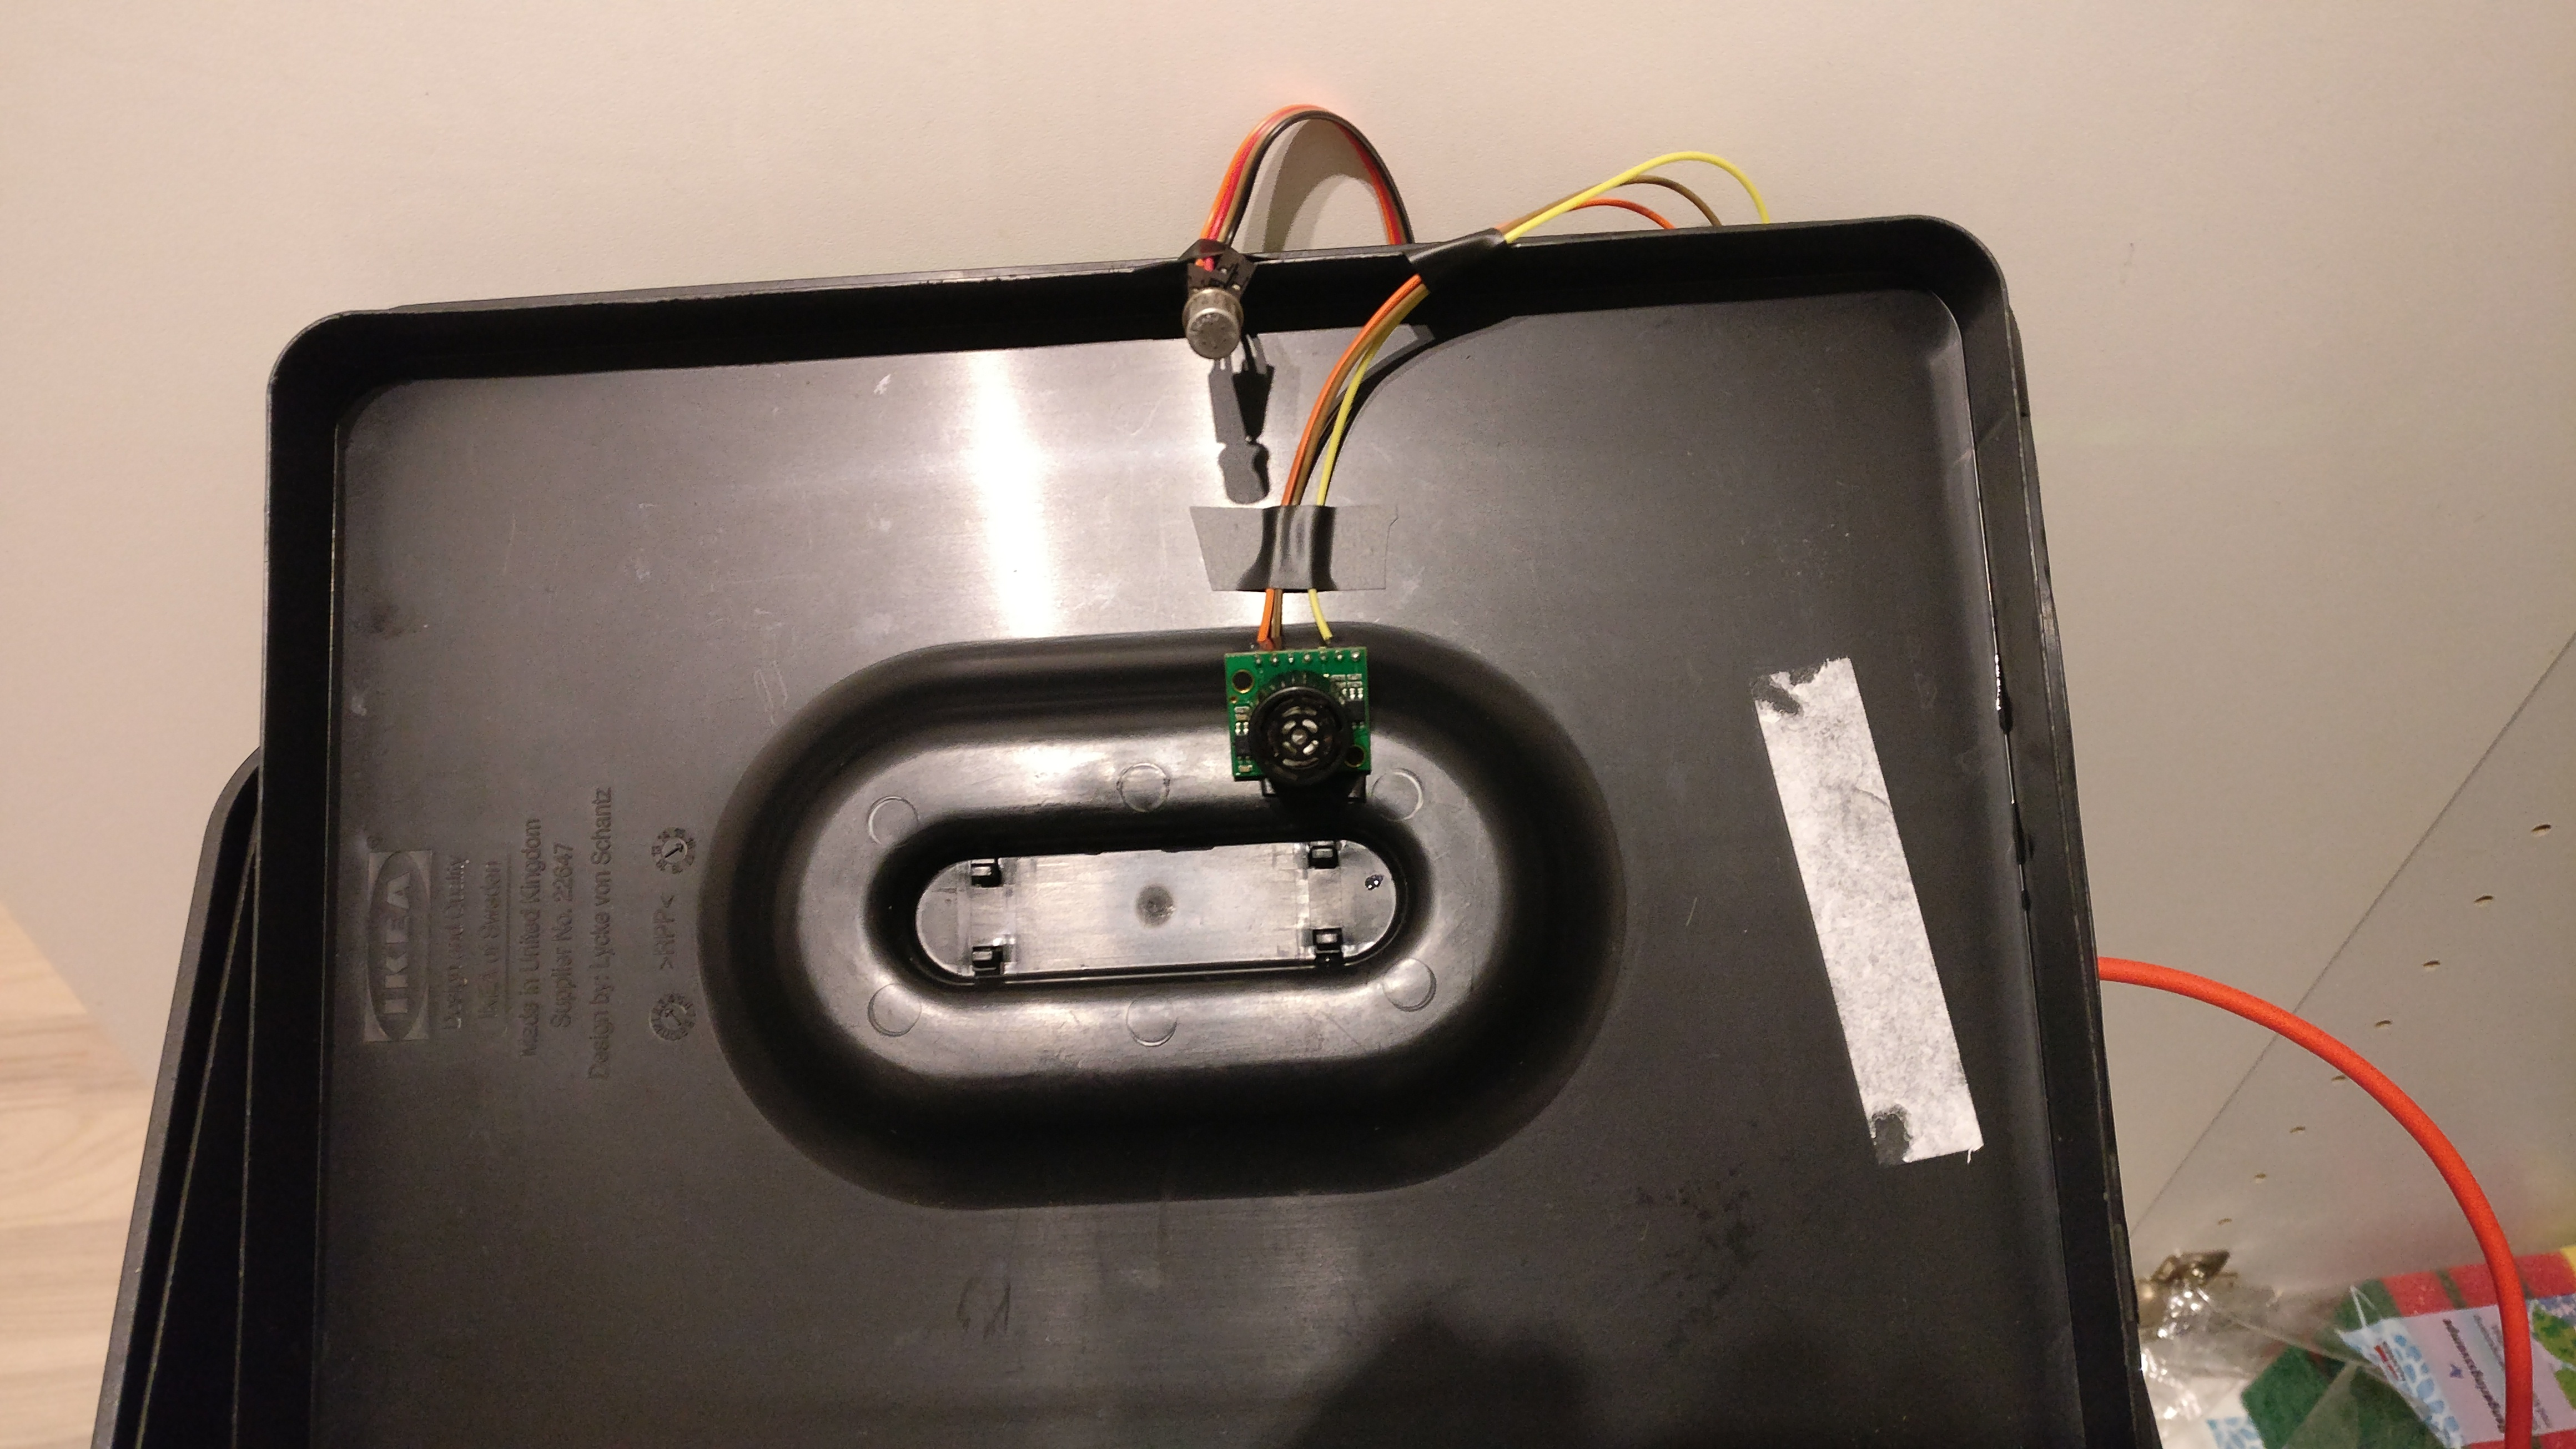
\includegraphics[scale=.05]{img/IMG_20161130_163302}
\caption{The sensors facing the inside of the bin.}
\label{fig:sensors}
\end{figure}

\subsection{Data layer}
The data layer is a simple RESTful web service for collecting the data and storing it in a database, thus making it accessible to potential consumers.

The service supports two types of entities, the SmartBins and the contexts.\\
Every SmartBin has a unique identifier and some information about its recent state information.\\
Every context is information about a state tied to a bin.\\
The REST api supports filtering of contexts by bin and lookups of all bins.

\subsection{Data Consumer}
The consumer in our case is an android client, but could just as easily have been any other platform able to connect to the internet and present content.

Our client can work in two separate modes: either as an android application or simply as an ambient display (single bin mode).

On the android application it is possible to manage multiple bins and get an overview of the last values measured by the system.

The ambient display is much more simple, it just displays a color of a shade from blue to red depending on the scent level, and the latest values measured for such bin.

In our system we use an android phone to run in both modes, so pressing on the screen even in ambient display mode will give the user the extra functionality of getting the overview for every bin that is registered to the user and of viewing the complete set of data measured from the bins.

Ideally the ambient display can be placed in a strategic location inside the house, for example by the door or on the fridge, where people can be reminded of the trash status and act accordingly.

Figure \ref{fig:interaction} shows an example of interaction with the ambient display.

\begin{figure}
\centering
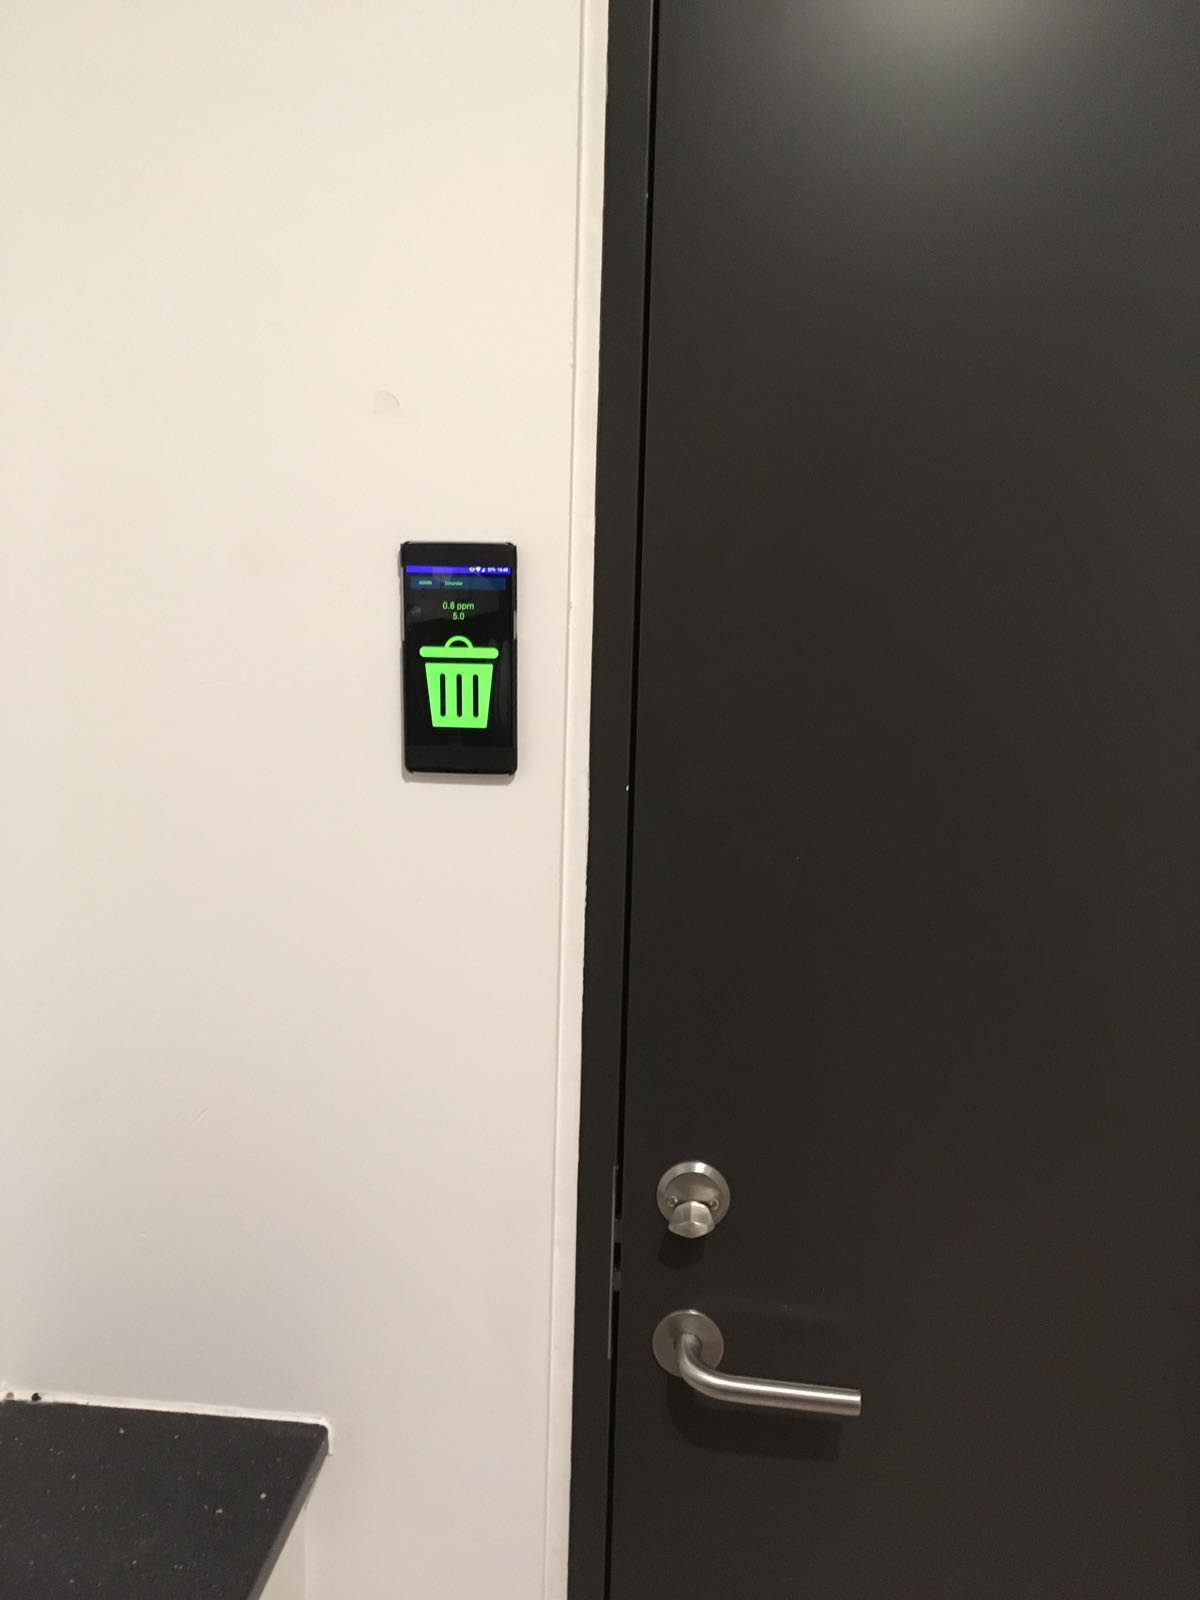
\includegraphics[scale=.05]{img/IMG-20161130-WA0000}
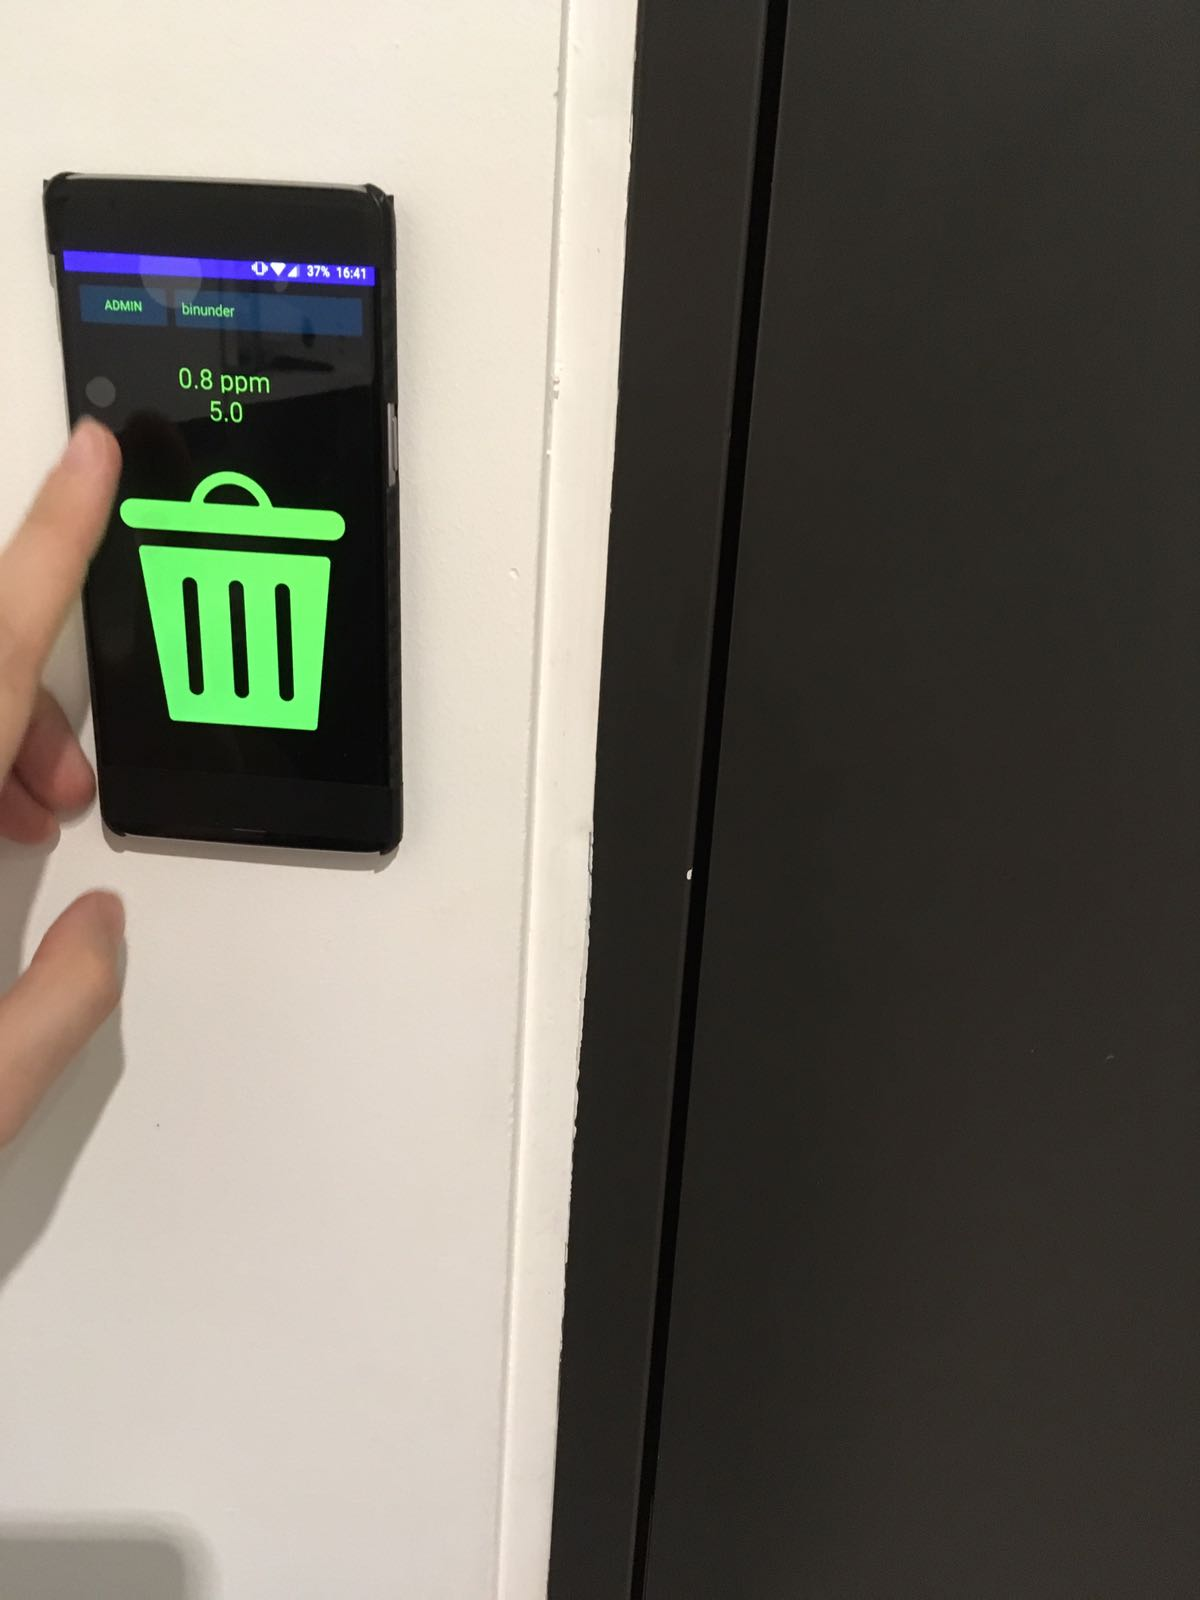
\includegraphics[scale=.05]{img/IMG-20161130-WA0004}
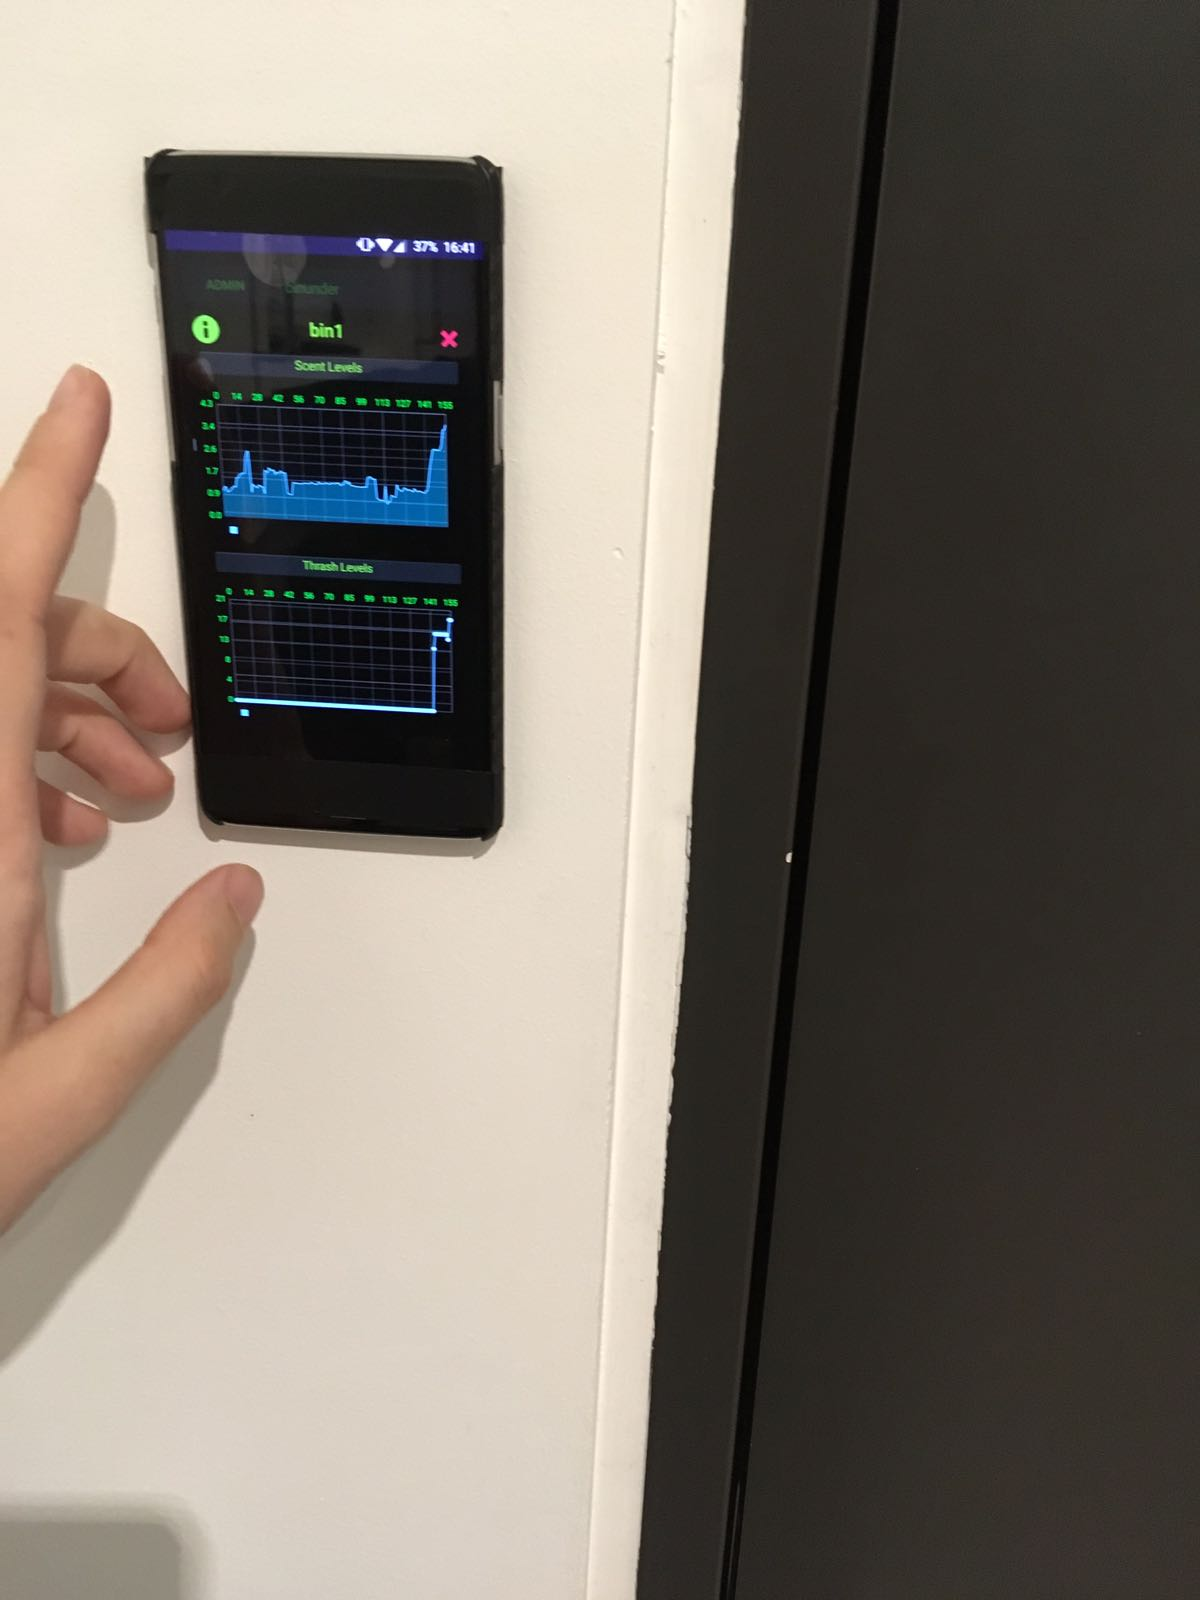
\includegraphics[scale=.05]{img/IMG-20161130-WA0002}
\caption{Interaction with ambient display}
\label{fig:interaction}
\end{figure}